\subsection*{Interferenz bei Lichtwellen}
Ziel dieses Versuchs ist die Messung der Wellenlänge eines Lasers und die Bestimmung der Brechzahlen von Luft und $\ce{CO2}$. Ganz zentral ist hierbei die Interferenz von Licht. \\
Für die Erklärung der Interferenz eignet sich die Beschreibung des Lichts als ebene, elektromagnetische Welle
\begin{align}\label{E-Feld}
	\vec{E}(x,t) = \vec{E}_0\cos(kx-\omega t-\delta)
\end{align}
am besten. Zur Beschreibung der Effekte ist die Betrachtung des elektrischen Feldes in einer Dimension, der Ausbreitungsrichtung $x$, ausreichend. Die restlichen Größen sind die Wellenzahl $k$, die (Kreis-)Frequenz $\omega$ und ein Phasenverschub $\delta$ bezogen auf einen festen Anfangspunkt. Treffen zwei Lichtwellen aufeinander können ihre Feldstärken einfach addiert werden. Das führt bei einem Gangunterschied von $2\pi n$ ($n\in\mathbb{N}$), zwischen den beiden Einzelwellen, zu einer Feldstärke
\begin{align*}
	\vec{E}_{ges}(x,t) &= \vec{E}_{10}\cos(kx-\omega t+2\pi n) + \vec{E}_{20}\cos(kx-\omega t) \\
	&= \left(\vec{E}_{10}+\vec{E}_{20}\right)\cos(kx-wt) \ ,
\end{align*}
bei einem Gangunterschied von $(2n+1)\pi$ dagegen ist die resultierende Gesamtfeldstärke
\begin{align*}
	\vec{E}_{ges}(x,t) &= \vec{E}_{10}\cos(kx-\omega t+(2n+1)\pi) + \vec{E}_{20}\cos(kx-\omega t) \\
	&= \left(\vec{E}_{20}-\vec{E}_{10}\right)\cos(kx-wt) \ .
\end{align*}
Haben die beiden Lichtstrahlen die gleiche Amplitude wird die Feldstärke verdoppelt bzw. komplett ausgelöscht. \\
Aufgrund der hohen Frequenz von sichtbarem Licht, ist es allerdings unmöglich die sich schnell ändernde Feldstärke zu messen, sodass im Experiment die Intensität
\begin{align}
	I = \frac{1}{t_2-t_1}\int_{t_1}^{t_2}\left|\vec{E}(x,t)\right|^2 \text{d}t
\end{align}
verwendet wird. Der Integrationszeitraum $t_2-t_1$ sollte dabei groß gegenüber der Periodendauer $\frac{2\pi}{\omega}$ sein. Für zwei sich überlagernde elektromagnetische Wellen (hier in komplexer Schreibweise, um die Rechnung zu vereinfachen) aus derselben Quelle (gleiche Amplitude und Frequenz) ist die Intensität dann
\begin{align}
	I &= \frac{\vec{E}_0^2}{t_2-t_1}\int_{t_1}^{t_2}\left|\mathrm{e}^{i(kx-\omega_t-\delta_1)}+\mathrm{e}^{i(kx-\omega t-\delta_2)}\right|^2 \text{d}t \\
	&= \frac{\vec{E}_0^2}{t_2-t_1}\int_{t_1}^{t_2}
	\left(2+2\cos(\delta_2-\delta_1)\right)
	\text{d}t \\
	&\label{Intensitat}= 2\vec{E}_0^2\left(1+\cos(\delta_2-\delta_1)\right) \ .
\end{align}
Sie liegt, abhängig vom Gangunterschied $\delta_2-\delta_1$, zwischen $0$ und $4\vec{E}_0^2$.
\subsection*{Voraussetzungen für die Beobachtung von Interferenz}
Bei alltäglichen Lichtquellen, wie der Sonne oder einer Glühbirne, sind die Parameter $\omega,k,\delta_1,\delta_2$ keine Konstanten. Dieses Licht hat keine feste Frequenz $\omega$, vielmehr sind verschiedene Frequenzen aus einem Frequenzbereich $\omega_0\pm\Delta \omega$ vertreten. Gleiches gilt für die Wellenlänge $\lambda=\frac{2\pi}{k}$. Da das Licht solcher Quellen spontan emittiert wird, sind die Phasenverschübe $\delta_1$ und $\delta_2$ statistische Funktionen der Zeit, sodass das Integral des Cosinus-Terms über eine lange Zeit $t_2-t_1$ verschwindet und eine konstante Intensität beobachtet wird. Aufgrund der nicht-konstanten Parameter ist dieses Licht nicht interferenzfähig und wird als inkohärent bezeichnet. Kohärentes Licht dagegen kann durch \emph{einen} Ausdruck \eqref{E-Feld} mit festen $k, \omega$ und $\delta$ beschrieben werden. \\
Üblicherweise wird ein Laser verwendet, wenn Licht mit hoher Kohärenz benötigt wird. Durch einen geeigneten Versuchsaufbau (siehe Abbildung \ref{Gluhlampe}) können allerdings auch bei eigentlich nichtkohärenten Lichtquellen Interferenz-Erscheinungen beobachtet werden.
\begin{figure}[h!]
	\centering
	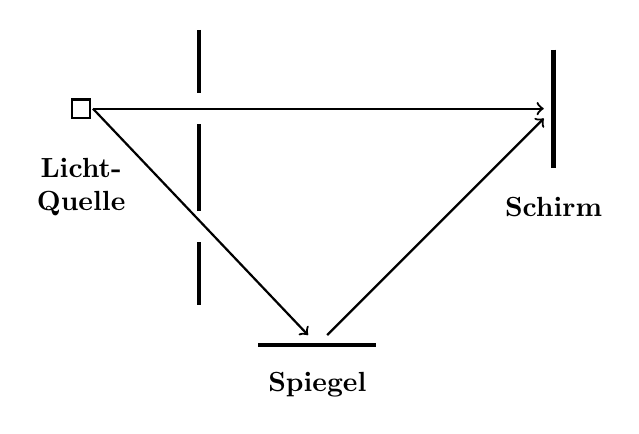
\begin{tikzpicture}
	\node(L)at(-3,0)[rectangle,draw,thick]{};
	\node(P)at(3,0){};
	\node(S)at(0,-3){};

%Beschriftung	
	\node(LQ)at(-3,-1)[align=center]{\textbf{Licht-}\\\textbf{Quelle}};
	\node(Box)at(0,-3.5){\textbf{Spiegel}};
	\node(K)at(3,-1.25){\textbf{Schirm}};
	
	\path [-, ultra thick]
	(-1.5,1)edge(-1.5,0.2)
	(-1.5,-0.2)edge(-1.5,-1.3)
	(-1.5,-1.7)edge(-1.5,-2.5)
	(3,0.75)edge(3,-0.75)         % Schirm
	(-0.75,-3)edge(0.75,-3);      % Spiegel
	
	\path [->, thick]
	(-2.85,0)edge(P)
	(-2.85,0)edge(S)
	(S)edge(P);
\end{tikzpicture}
	\caption{Versuchsaufbau, der eine nicht interferenzfähige Lichtquelle für Interferenz-Experimente erlaubt}
	\label{Gluhlampe}
\end{figure} 
Hierbei wird das Licht in zwei Teilstrahlen geteilt, die so umgelenkt werden, dass sie am Schirm wieder aufeinander treffen. Um dort Interferenzeffekte beobachten zu können muss das Frequenzspektrum schmal sein, da es sonst beispielsweise zu einer Auslöschung kommen kann, obwohl zwei Wellen zu einem vorigen Zeitpunkt in Phase waren. Zudem ist wichtig, dass der Emissionsvorgang nicht instantan passiert, sondern eine endliche Zeit $\tau$ dauert, woraus eine endliche Länge $l$ des Paketes resultiert. Aber nur Wellenpakete, die zur selben Zeit am Schirm auftreffen können interferieren. Deshalb darf der Wegunterschied zweier Strahlen, die unterschiedliche Wege zum Schirm genommen haben, nicht größer als die Koherenzlänge $l$ sein.